% !TeX root = report_example.tex
\newcommand*{\PathToAssets}{../assets}%
\newcommand*{\PathToOutput}{../_output}%
% \newcommand*{\PathToBibFile}{bibliography.bib}%


%%%%%%%%%%%%%%%%%%%%%%%%%%%%%%%%%%%%%%
%% This file is compiled with XeLaTex.
%%%%%%%%%%%%%%%%%%%%%%%%%%%%%%%%%%%%%%
\documentclass[12pt]{article}
%\documentclass[reqno]{amsart}
%\documentclass[titlepage]{amsart}
\usepackage{my_article_header}
\usepackage{my_common_header}

\begin{document}
\title{
Replicating TIPS-Treasury Arbitrage from \cite{SegmentedArb}
%\\{\color{blue} \large Preliminary Idea Write-up}
}
% {\color{blue} \large Preliminary. Do not distribute.}
% }

\author{
Bailey Meche\footnote{University of Chicago}, 
Raul Renteria\footnote{University of Chicago}
  % \newline 
  % \hspace{3pt} \indent \hspace{3pt}
  % % I am immensely grateful to...
}
% \maketitle
\begin{titlepage}
% \input{cover_letter.tex}
\maketitle
%http://tex.stackexchange.com/questions/141446/problem-of-duplicate-identifier-when-using-bibentry-and-hyperref
% \nobibliography*

% Abstract should have fewer than 150 words

\doublespacing
\begin{abstract}
  In this report, we replicate the TIPS–Treasury arbitrage strategy over the period 2010–2020, 
  following the methodology of \cite{Fleckenstein} as described in \cite{SegmentedArb}. Our objective is to determine whether the mispricing 
  puzzle they documented – wherein nominal Treasury bonds appear overpriced relative to inflation-protected Treasuries (TIPS) 
  after accounting for inflation swap rates – persisted into the 2010s. We construct a synthetic nominal Treasury 
  yield from TIPS and inflation swap contracts and compare it to the actual nominal Treasury yield of the same maturity. 
  Our findings indicate that a positive arbitrage spread (Treasury yield lower than its synthetic counterpart) persisted 
  throughout 2010–2020, though the magnitude of this mispricing is smaller than that reported in the mid-2000s. The arbitrage
   opportunity gradually narrowed over the decade, consistent with increasing market efficiency or capital flowing into the trade, 
   yet it did not fully disappear. These results reinforce the notion that significant pricing discrepancies can endure in large, 
   liquid markets, highlighting the role of market frictions and slow-moving arbitrage capital in sustaining such inefficiencies.
\end{abstract}


\end{titlepage}

\doublespacing
\section{Introduction}

The coexistence of nominal Treasury bonds and Treasury Inflation-Protected Securities (TIPS) offers a natural test of the law of one price. 
In theory, one can combine a TIPS (which provides real cash flows adjusted for inflation) with an inflation swap to exactly replicate the 
cash flows of an ordinary nominal Treasury bond. Under frictionless and efficient markets, the price of this synthetic Treasury should equal the 
price of an actual Treasury bond of equivalent maturity. However, \cite{Fleckenstein} revealed a persistent deviation from 
this parity, now widely known as the TIPS–Treasury puzzle. They found that nominal Treasury bonds were almost always overpriced relative to TIPS after adjusting for inflation 
expectations. In some cases, a Treasury’s price exceeded that of an inflation-swapped TIPS by more than \$20 per \$100 of face value. 
This gap corresponded to yield differentials on the order of dozens of basis points, with an average mispricing of about 55 basis points and peaks 
over 200 basis points in the 2004–2009 sample. 
Such a large and systematic arbitrage spread – vastly exceeding typical anomalies like the 5–10 basis point on-the-run/off-the-run Treasury premium 
 – represents one of the largest arbitrage opportunities documented in fixed-income markets, posing a challenge to classical asset pricing theory.

This TIPS–Treasury arbitrage is significant not only for its size but also for what it reveals about market efficiency and limits of arbitrage. 
A persistent price discrepancy in two of the world’s deepest bond markets suggests that certain investors face constraints or frictions that prevent 
immediate arbitrage correction. \cite{Fleckenstein} provide evidence that as capital flowed into arbitrage trades, the mispricing narrowed, 
supporting a “slow-moving capital” explanation. The idea is that arbitrage capital may not instantly rush in to eliminate mispricing; instead, it adjusts gradually due to 
investor constraints, risk aversion, or institutional frictions. This perspective builds on the limits-to-arbitrage literature \citep{Shleifer1997-py} 
which shows that even textbook arbitrage opportunities can persist when arbitrageurs are risk- or capital-constrained 
\citep{Fleckenstein}. In this context, the TIPS–Treasury puzzle serves as a real-world case study of how market segmentation and funding 
constraints allow a seemingly free lunch to continue over time.

In this report, we replicate the TIPS–Treasury arbitrage analysis for the period 2010–2020. Extending the sample beyond \cite{Fleckenstein}’s 2004–2009 
window allows us to examine whether the pricing gap continued in the subsequent decade and how it evolved through varying market conditions (e.g., 
the post-financial-crisis recovery, periods of unconventional monetary policy, and the lead-up to the COVID-19 crisis). We follow the original 
methodology closely to construct the arbitrage spread, and we analyze its behavior relative to the earlier findings. By doing so, we shed light on 
whether arbitrage opportunities in this market have been corrected by the 2010s or whether frictions still permitted economically significant 
mispricings. Our analysis contributes to the literature on asset pricing anomalies and market efficiency, confirming that the TIPS–Treasury mispricing,
 while reduced, remained a notable feature of the market in the 2010–2020 period.



%I give an example of a simple table in Table \ref{table:tips_treasury_summary_table.tex}.





\section{Model}
%# Methodology  
%## Replicating the Synthetic Nominal Treasury Yield  
We replicate the arbitrage strategy as described by \cite{Fleckenstein} by constructing a synthetic nominal Treasury yield. 
The key steps are as follows:  

\begin{enumerate}
  \item Data Collection
  \begin{itemize}
    \item TIPS Data: Daily yield data for TIPS, obtained from U.S. Treasury sources, provide the real yield (adjusted for inflation).  
    \item Inflation Expectations Data: Zero-coupon inflation rates for corresponding maturities are sourced from the Cleveland Fed's Term Structure of Inflation Expectations release.
    \item Nominal Treasury Data: Daily yields for nominal Treasuries are obtained from CRSP.  
  \end{itemize}
  

  \item Synthetic Yield Construction
  For a given maturity \(\tau\), let
  \begin{itemize}
    \item \(s_{t,\tau}\) be the TIPS yield (the real yield) at time \(t\).
    \item  \(f_{t,\tau}\) be the fixed rate on an inflation swap for the same maturity.
    \item  \(y_{T,t,\tau}\) be the yield on a nominal Treasury bond.
  \end{itemize} 
\end{enumerate}
The synthetic nominal yield is then given by:
\[
\text{Synthetic Yield}_{t,\tau} = s_{t,\tau} + f_{t,\tau}.
\]
The TIPS–Treasury arbitrage spread is defined as:
\[
\text{Spread}_{t,\tau} = (s_{t,\tau} + f_{t,\tau}) - y_{T,t,\tau}.
\]
A positive spread indicates that nominal Treasuries are yielding less (i.e., priced higher) than the synthetic security, 
signaling a potential arbitrage opportunity.


%## Practical Implementation of the Arbitrage Strategy  
In addition to the replication exercise, I outline below how a trader would implement this strategy in practice:
\begin{itemize}
  \item Identifying the Opportunity:  
  
  The trader continuously monitors the daily yields for TIPS, inflation swaps, and nominal Treasuries. By computing the synthetic yield \(s_{t,\tau} + f_{t,\tau}\) and comparing it to the observed nominal Treasury yield \(y_{T,t,\tau}\), the trader identifies when the arbitrage spread is positive. A consistently positive spread suggests that nominal Treasuries are overvalued relative to their inflation-protected counterparts.

  \item  Position Construction:  
  
  When a positive spread is detected, the trader would:
  
  \begin{itemize}
    \item Go Long on TIPS: Purchase TIPS of the desired maturity.
    \item Enter into Inflation Swaps: Execute zero-coupon inflation swap contracts with maturities matching those of the TIPS cash flows. These swaps convert the inflation-adjusted (real) cash flows of TIPS into fixed nominal cash flows.
    \item Short the Nominal Treasury: Simultaneously, short the nominal Treasury bond with the same maturity. Alternatively, if shorting physical bonds is not practical due to market constraints, the trader could use Treasury futures or repurchase agreements (repos) to synthetically short the nominal bond.
  \end{itemize} 
  \item Cash Flow Matching and Hedging:  
  
  The trader may use Treasury STRIPS or other derivatives to fine-tune the cash flow replication. This ensures that the cash flows from the long TIPS position (adjusted via the inflation swap) exactly offset those from the short nominal Treasury. The goal is to lock in the arbitrage spread as a risk-free profit, with minimal exposure to market movements in yields or inflation.

  \item Risk Management and Execution:  

  Although the theoretical spread represents a “riskless” arbitrage, practical implementation involves risks such as mark-to-market volatility, liquidity risk, and execution costs (e.g., bid-ask spreads and margin requirements). The trader must:
  \begin{itemize}
    \item Monitor Margins and Collateral: Regularly review margin calls and maintain sufficient collateral in both the bond and swap positions.
    \item Manage Counterparty Risk: Ensure that counterparties in the inflation swaps and repurchase agreements are creditworthy.
    \item Hedge Residual Exposures: In cases where exact cash flow matching is not possible, use additional hedging instruments (such as interest rate derivatives) to manage residual risks.
  \end{itemize} 
  
  \item Capital and Funding Considerations. 
  The strategy typically requires significant capital, as the trader must finance the TIPS purchase while potentially borrowing against short positions. Funding costs, including any constraints on borrowing, can affect the net profit of the arbitrage. As noted in previous literature, slow-moving capital may delay the full exploitation of the arbitrage opportunity.

%By following these steps, a trader can systematically exploit the mispricing between nominal Treasuries and their synthetic counterparts. The persistent positive spread offers a recurring signal for potential profit, though careful management of the associated risks is crucial for success.

\end{itemize}

\section{Results}
%\subsection{Series}
%\subsection{Summary Statistics}
 Table \ref{table:tips_treasury_summary_table.tex} presents summary statistics for the daily TIPS–Treasury arbitrage spread from 2010 to 2020. 
 \begin{table}
  %\caption{A Simple Table From Pandas, No. 1}
  \centering
  \begin{tabular}{lllll}
\toprule
 & TIPS-Treasury 2Y & TIPS-Treasury 5Y & TIPS-Treasury 10Y & TIPS-Treasury 20Y \\
\midrule
Mean & 20 & 19 & 25 & 26 \\
p50 & 23 & 20 & 25 & 26 \\
Std. Dev & 14 & 8 & 7 & 8 \\
Min & 0 & 0 & 0 & 1 \\
Max & 54 & 56 & 40 & 47 \\
AR1 & 0.978 & 0.981 & 0.976 & 0.974 \\
First & Jan-2010 & Jan-2010 & Jan-2010 & Jan-2010 \\
Last & Feb-2020 & Feb-2020 & Feb-2020 & Feb-2020 \\
N & 2506 & 2541 & 2541 & 2541 \\
\bottomrule
\end{tabular}

  \caption{
    Summary Statistics of TIPS–Treasury Arbitrage Spread, 2010–2020
  }
  \label{table:tips_treasury_summary_table.tex}
  \end{table}
 The statistics confirm that the mispricing, while smaller than in the mid-2000s, remained economically significant. 
 The mean spread over this period is on the order of a few tens of basis points, indicating that on an average day, the Treasury yield was around 
 0.2–0.3\% lower than the synthetic yield. The median spread is of similar magnitude, suggesting the distribution of the spread is fairly symmetric 
 around a positive value. The standard deviation is also on the order of a few basis points, reflecting noticeable variability in the arbitrage over 
 time. The spread is consistently positive – the minimum daily value recorded in our sample is still a positive single-digit number of basis points, 
 while the maximum spread reached around half a percentage point. These figures can be compared to those documented by \cite{Fleckenstein}. for 
 2004–2009: they found an average spread of ~54.5 bps and much higher volatility \citep{Fleckenstein}. The smaller average mispricing in 
 2010–2020 suggests that the gap between TIPS and Treasury pricing has narrowed, but not vanished. Importantly, the fact that the minimum spread 
 remained above zero implies there were virtually no instances in the 2010s where TIPS were rich relative to Treasuries – consistent with
  \cite{Fleckenstein}’s finding that Treasuries tend to be the overvalued side almost without exception.
 
%Time-Series Behavior: *
Figure \ref{fig:spreads} plots the evolution of the 10-year TIPS–Treasury arbitrage spread over time. 
\begin{figure}
  \centering
  \caption{Example plot}
    \centering
    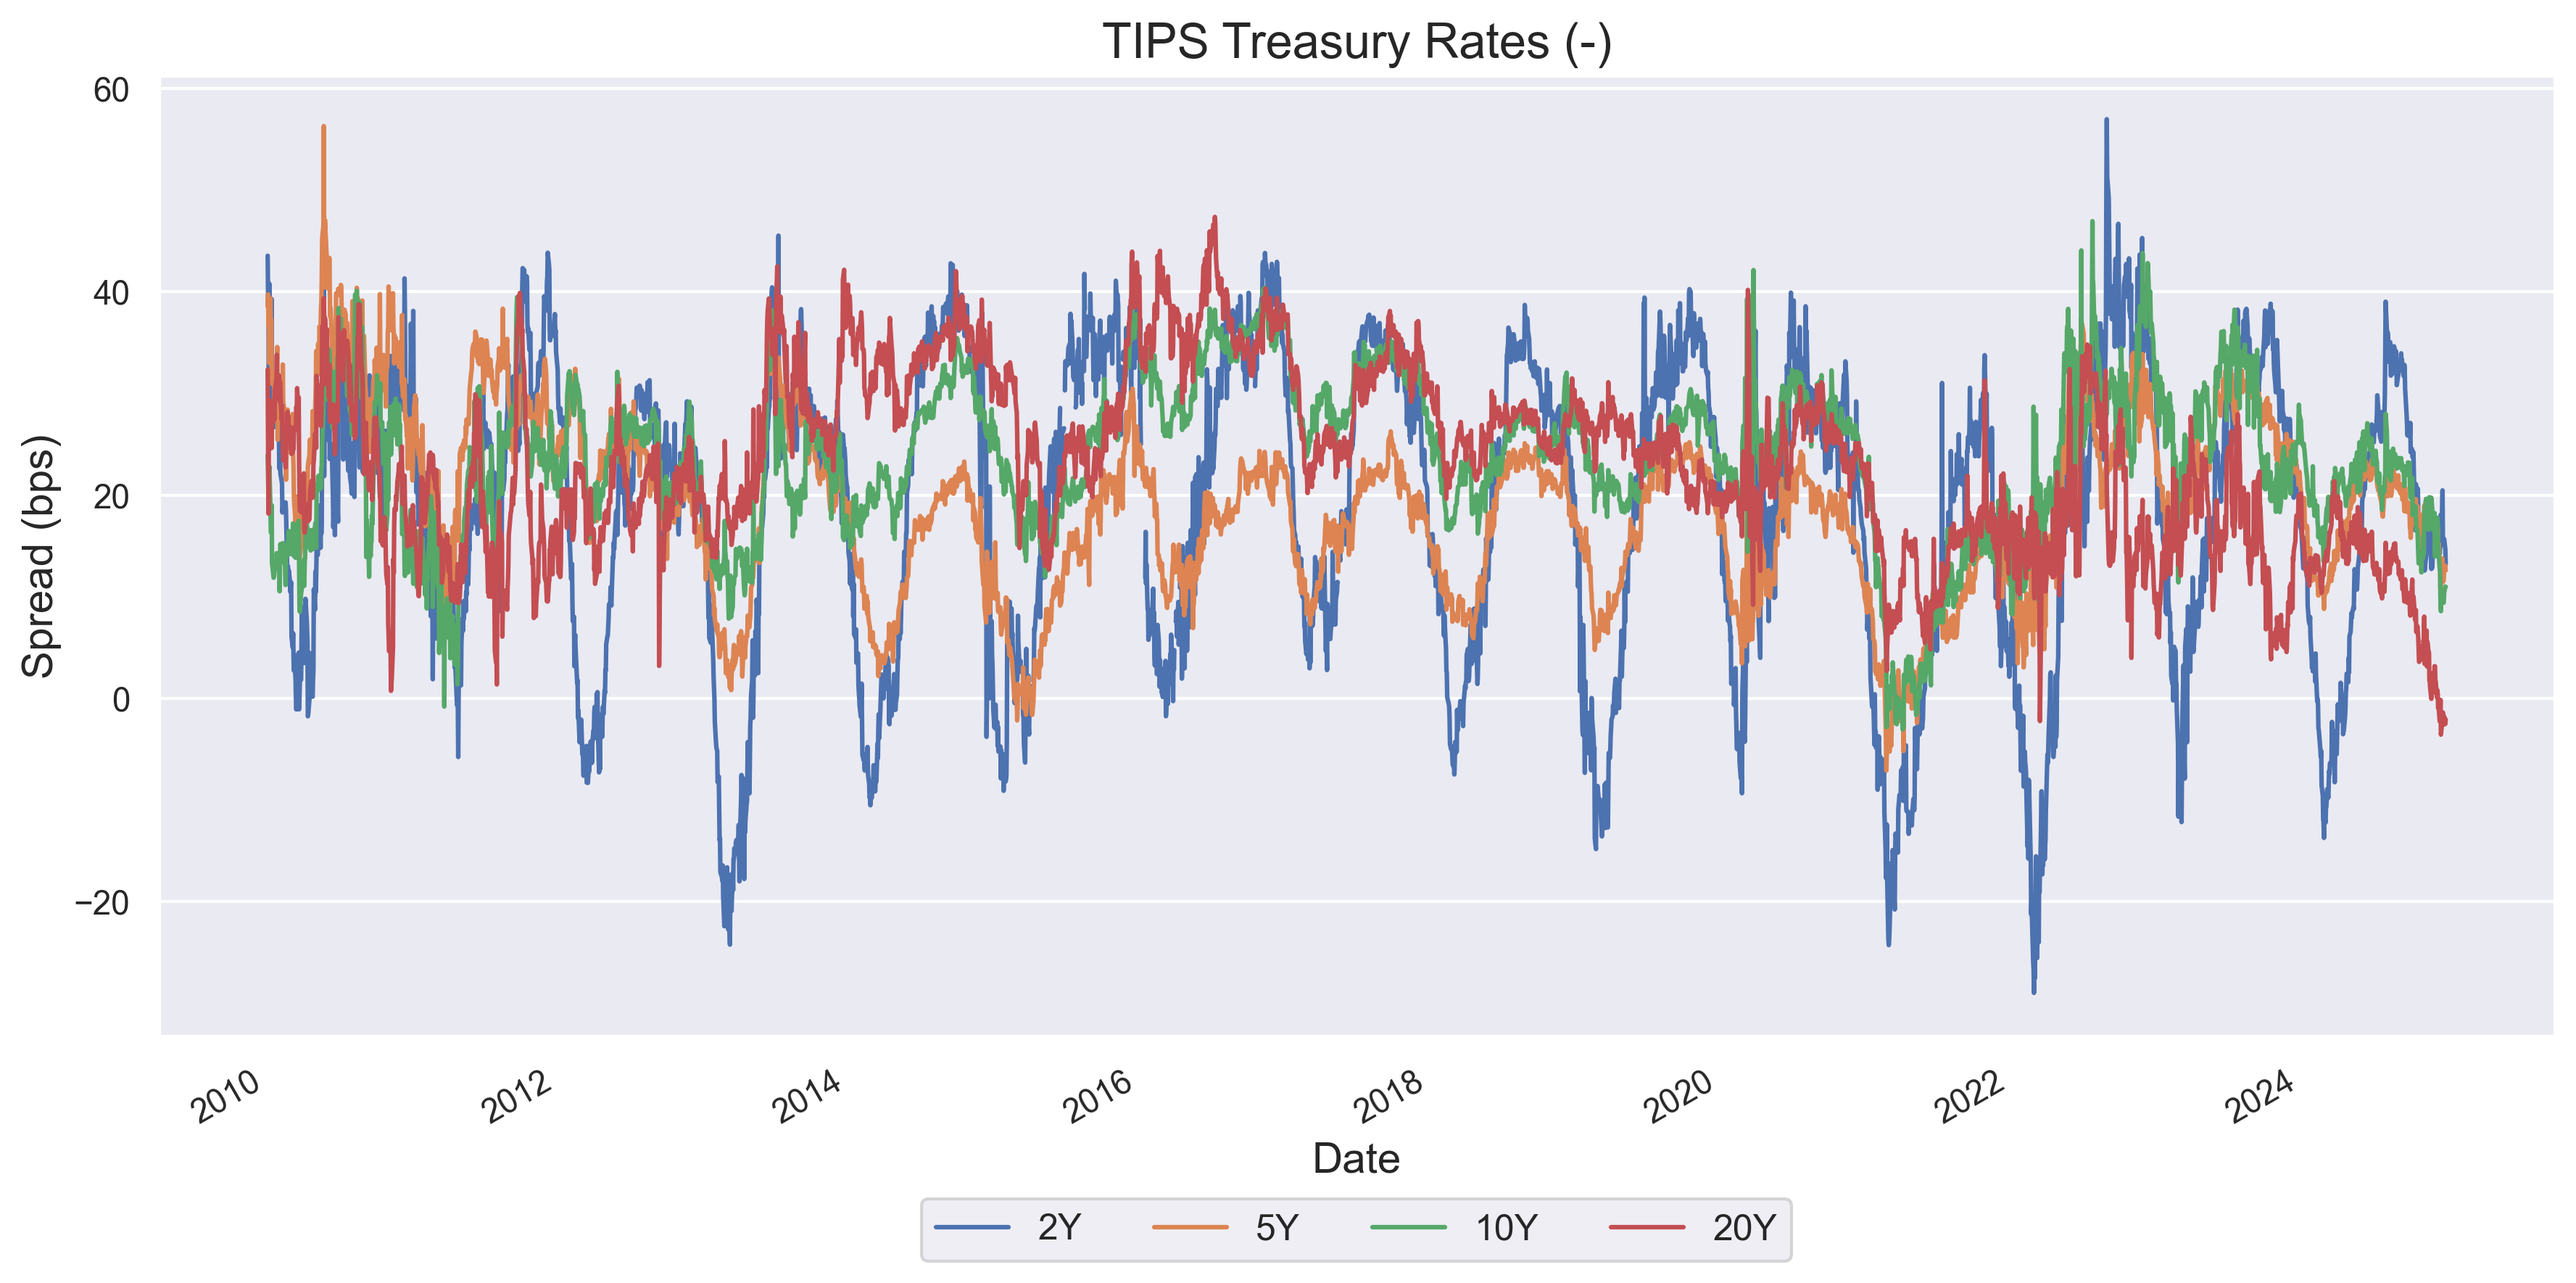
\includegraphics[width=\linewidth]{\PathToOutput/tips_treasury_spreads.png}
    \caption{TIPS–Treasury arbitrage spread, 2010–2020}
  \caption*{
    Inflation and Real GDP...
    }
  \label{fig:spreads}
  \end{figure}
  The time-series shows several notable trends. In the early 2010s (immediately after the 2008–09 financial crisis period covered by the original 
  study), the arbitrage spread started at elevated levels but showed a declining trend. This decline is consistent with the idea that as markets 
  normalized post-crisis and as more capital likely entered the trade, the mispricing shrank. By the mid-2010s, the spread oscillated at a moderate 
  level (on the order of 20–30 bps), still indicating Treasuries were comparatively expensive, but the gap was substantially smaller than the peaks 
  observed during the crisis. There were intermittent fluctuations – for example, around mid-2013, some volatility corresponds to the “taper tantrum” 
  period; during such episodes of market stress, we see modest widening of the spread as TIPS may have become relatively cheaper (possibly due to 
  liquidity differences or flight-to-quality flows favoring nominals). The general pattern from 2010 to 2019 is one of a slowly mean-reverting spread 
  that never fully closes. Arbitrageurs earned a positive carry throughout, but the opportunity was less dramatic than the mid-2000s heyday.

In late 2019 and into early 2020, the spread began to widen again. The onset of the COVID-19 pandemic and the associated market turmoil in March 
2020 led to a significant dislocation in the TIPS market: investors flocked to nominal Treasuries as a safe haven, while TIPS saw their prices drop 
(and yields spike) amid concerns about deflation and a dash for liquidity. Consequently, our arbitrage spread spiked sharply during March 2020,
 reaching levels not seen since the financial crisis. For instance, on certain days in March 2020, the 10-year TIPS yield jumped far above the n
 ominal yield once adjusted for collapsing inflation expectations, implying an arbitrage spread potentially well into the hundreds of basis p
 oints on an annualized basis (though these extreme values were short-lived). Figure \ref{fig:spreads} captures this spike clearly, showing a 
 pronounced jump in the spread. After the Federal Reserve’s interventions and restoration of market functioning, the spread contracted quickly by 
 mid-2020, though it remained somewhat higher than pre-COVID levels for a time. This episode underscores that even a decade after the initial 
 puzzle was documented, severe market stress can resurface the arbitrage gap in force.

Comparing our replicated results to \cite{Fleckenstein}, we observe the same qualitative phenomenon: nominal Treasuries have 
generally been overpriced relative to TIPS, and the mispricing persists over multi-year periods. The magnitude in the 2010s was lower on average 
than in the 2000s, which aligns with the original authors’ conjecture that additional capital would gradually arbitrage away the discrepancy 
\citep{Fleckenstein}. Indeed, by the 2010s the average spread of roughly 20–30 bps is about half of what was reported for the prior decade, 
suggesting a partial convergence toward no-arbitrage pricing. However, the continued presence of a non-zero (and sometimes large) spread – 
especially the flare-ups during turmoil – shows that the puzzle was not fully resolved. Market participants in the 2010s could still find 
opportunities to profit from this spread, although the window for extreme profits (like the >50 bp spreads pre-2010) had narrowed. In sum, 
our results confirm that the TIPS–Treasury arbitrage, while less pronounced than before, remained a meaningful anomaly throughout 2010–2020.


%%%%%%%%%%%%%
\subsection{Conclusion}  
In conclusion, our replication study finds that the TIPS–Treasury arbitrage identified by \cite{Fleckenstein} persisted into the 2010–2020 period, 
albeit at reduced levels. Using a first-principles construction of synthetic nominal Treasury yields from TIPS and inflation swaps, we consistently 
observe nominal Treasuries priced richer than their inflation-protected counterparts. The arbitrage spreads averaged a few dozen basis points in the 
2010s and never completely closed, indicating that arbitrage opportunities in this market endured. This persistence suggests that, even in highly 
liquid and closely watched markets, frictions can prevent perfect price alignment.

The gradual narrowing of the mispricing over the decade is a noteworthy finding. It hints at improving market efficiency: as awareness of the 
trade grew and more arbitrage capital entered (from hedge funds, proprietary trading desks, etc.), the pricing gap shrank compared to the mid-2000s. 
This is consistent with the slow-moving capital hypothesis – capital did flow in to reduce the arbitrage, but only slowly and partially 
\citep{Fleckenstein}. Periods of large dislocation (such as the COVID-19 shock) saw the spread widen dramatically again, only to tighten once 
normalcy returned, reinforcing the notion that liquidity and funding constraints play a pivotal role. In other words, when markets are under 
stress or when arbitrageurs face binding constraints, mispricings can widen and persist; when conditions normalize and capital is available, 
those mispricings tend to contract.

Our findings have important implications for market efficiency and arbitrage. The existence of a sustained TIPS–Treasury price discrepancy 
challenges the strictest form of efficient markets – it is effectively a \$100 bill lying on the sidewalk that took years to be mostly picked up. 
That it persisted underscores the real-world limits of arbitrage: factors such as regulatory constraints, balance sheet costs, risk aversion, and 
funding availability can prevent even large, near-arbitrage opportunities from being immediately exploited \citep{Fleckenstein}. 
This case echoes other instances in financial markets where theoretical arbitrages endured 
(e.g., covered interest parity deviations or CDS-bond bases), all pointing to the importance of intermediary constraints and segmented markets. 

In summary, the TIPS–Treasury arbitrage from 2010 to 2020 provides a striking example of how market inefficiencies can 
linger and slowly correct rather than instantaneously vanish. From a policy and practitioner standpoint, the continued (if diminishing) 
arbitrage spread suggests that improvements in market design and liquidity (such as expanding the investor base for TIPS or easing short-selling of 
Treasuries) could further enhance pricing efficiency. For academic finance, our replication affirms the conclusions of \cite{Fleckenstein}
over an extended sample: substantial arbitrage opportunities can exist even in government bond markets, and their resolution (or lack thereof) 
offers valuable insights into the mechanisms of market adjustment and the limits faced by arbitrageurs. The TIPS–Treasury puzzle thus remains a 
pertinent illustration of the interplay between arbitrage capital and market efficiency in the post-2008 financial landscape. 




% \begin{mydefinition}[Fibration]
%   A fibration is a mapping between two topological spaces that has the homotopy lifting property for every space \(X\).
% \end{mydefinition}

% \begin{proposition}
%   Let \(f\) be a function whose derivative exists in every point, then \(f\) is 
%   a continuous function.
% \end{proposition}
% \begin{proof}
%   We have that \(f\) is a differentiable function and so it must be continuous.
% \end{proof}

% \begin{mylemma}
%   Given two line segments whose lengths are \(a\) and \(b\) respectively there is a 
%   real number \(r\) such that \(b=ra\).
% \end{mylemma}

% \begin{proof}
%   To prove it by contradiction try and assume that the statement is false,
%   proceed from there and at some point you will arrive to a contradiction.
% \end{proof}




\newpage
\bibliographystyle{jpe}
\bibliography{bibliography.bib}  % list here all the bibliographies that you need. 
% \bibliography{\PathToBibFile}
% \printbibliography

% \newpage
% \begin{appendices}
% \section{Proofs}

% TODO



% \section{Recycle Bin}
% {\textbf{(Short-term parking spot for material that may be re-used or deleted at a later time)}}


% TODO

% \end{appendices}
\end{document}
